\documentclass[border=2pt]{standalone}
\usepackage{tikz}
\usetikzlibrary{arrows.meta,topaths}

\begin{document}
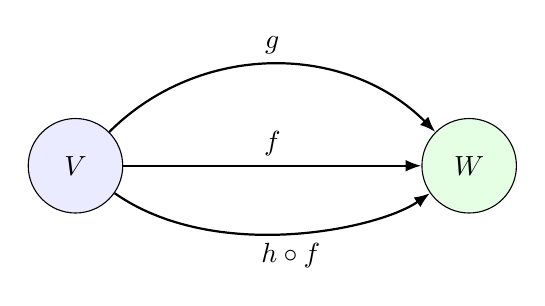
\begin{tikzpicture}[
  object/.style={draw,circle,minimum size=12mm,inner sep=1pt},
  morphism/.style={-{Latex[length=2mm]},thick}
]
  \node[object,fill=blue!8] (V) at (0,0) {$V$};
  \node[object,fill=green!10] (W) at (5,0) {$W$};

  \path[morphism]
    (V) edge node[above] {$f$} (W)
    (V) edge[min distance=13mm] node[above] {$g$} (W)
    (V) edge[out=-35,in=-145,out min distance=7mm,in max distance=8mm]
      node[below] {$h\circ f$} (W);
\end{tikzpicture}
\end{document}
